\section*{4}
\subsection*{4.1}
Pauli-Dirac表示を用いると,
\begin{equation}
  \vec{\alpha}_i = 
  \begin{pmatrix}
    0 & \sigma_i \\
    \sigma_i & 0 \\
  \end{pmatrix}
  , \qquad
  \beta = 
  \begin{pmatrix}
    I & 0 \\
    0 & -I \\
  \end{pmatrix}
\end{equation}
と書ける.
ただし,$\sigma_i\,(i=1,2,3)$はPauli行列,$I$は$2\times 2$の単位行列を表す.
一方,
\begin{equation}
  S_z = 
  \begin{pmatrix}
    \sigma_3 & 0 \\
    0 & \sigma_3 \\
  \end{pmatrix}
\end{equation}
と書ける.
したがって,
\begin{align}
  \left[H_D, S_z\right] &= \left[\sum_i \alpha_i p_i + \beta m, S_z\right] \notag\\
  &= \sum_i \left[
    \begin{pmatrix}
      0 & \sigma_i \\
      \sigma_i & 0 \\
    \end{pmatrix}  
    ,
    \begin{pmatrix}
      \sigma_3 & 0 \\
      0 & \sigma_3 \\
    \end{pmatrix}
  \right]
  p_i +  \left[
    \begin{pmatrix}
      I & 0 \\
      0 & -I \\
    \end{pmatrix}
    ,
    \begin{pmatrix}
      \sigma_3 & 0 \\
      0 & \sigma_3 \\
    \end{pmatrix}
  \right]
  m \notag \\
  &= 
  \begin{pmatrix}
    0 & [\sigma_x,\sigma_z]p_x + [\sigma_y, \sigma_z]p_y \\
    [\sigma_x,\sigma_z]p_x + [\sigma_y, \sigma_z]p_y & 0 \\
  \end{pmatrix} \notag\\
  &= i 
  \begin{pmatrix}
    0 & \sigma_x p_y -\sigma_y p_x\\
    \sigma_x p_y -\sigma_y p_x & 0 \\
  \end{pmatrix} \neq 0
\end{align}
と計算できる.
ただし,最後の変形で
\begin{equation}
  [\sigma_i, \sigma_j] = i\epsilon_{ijk}\sigma_k
\end{equation}
を用いた.
したがって,$H_D$と$S_z$は可換ではない.

\subsection*{4.2}
\begin{equation}
  h = \frac{2\vec{S}\vec{p}}{\left|\vec{p}\right|} = \frac{2}{\left|\vec{p}\right|}
  \sum_j
  \begin{pmatrix}
    \sigma_j & 0 \\
    0 & \sigma_j \\
  \end{pmatrix}
  p_j
\end{equation}
より,
\begin{align}
  [H_D, h] &= \frac{2}{\left|\vec{p}\right|} \sum_{i,j} \left[
  \begin{pmatrix}
    0 & \sigma_i \\
    \sigma_i & 0 \\
  \end{pmatrix}
  ,
  \begin{pmatrix}
    \sigma_j & 0 \\
    0 & \sigma_j \\
  \end{pmatrix}
  \right] p_i p_j + \frac{2}{\left|\vec{p}\right|} \sum_j
  \left[
  \begin{pmatrix}
    I & 0 \\
    0 & -I \\
  \end{pmatrix}
  ,
  \begin{pmatrix}
    \sigma_j & 0 \\
    0 & \sigma_j \\    
  \end{pmatrix}
  \right] p_j\notag\\
  &= \frac{2}{\left|\vec{p}\right|} \sum_{i,j}
  \begin{pmatrix}
    0 & [\sigma_i,\sigma_j] \\
    [\sigma_i,\sigma_j] & 0 \\
  \end{pmatrix}
  p_i p_j \notag\\
  &= \frac{2}{\left|\vec{p}\right|} \sum_{i,j} i \epsilon_{ijk}
  \begin{pmatrix}
    0 &  \sigma_k\\
    \sigma_k & 0 \\
  \end{pmatrix}
  p_i p_j \notag\\
  &= \frac{2}{\left|\vec{p}\right|} \sum_{i,j} i \frac{\epsilon_{ijk}-\epsilon_{jik}}{2}
  \begin{pmatrix}
    0 &  \sigma_k\\
    \sigma_k & 0 \\
  \end{pmatrix}
  p_i p_j \notag\\
  &= 0
\end{align}
と計算できる.
よって,$H_D$と$h$は可換である.

\section*{5}
ここではPauli-Dirac表示を用いる.
一般にスピノル$\psi$に対して
\begin{equation}
  \bar{\psi} = \psi^{\dagger}\gamma^0 = \psi^{\dagger}
  \begin{pmatrix}
    I & 0 \\
    0 & -I \\
  \end{pmatrix}
\end{equation}
であることを用いると,
\begin{align}
  \sum_i u_i \bar{u}_i 
  &= \sum_{a=A,B} N^2 
  \begin{pmatrix}
    u_a \\ \frac{\vec{\sigma}\cdot \vec{p}}{E+m} u_a \\
  \end{pmatrix}
  \left(u_a^{\dagger}, \frac{\vec{\sigma}\cdot \vec{p}}{E+m} u_a^{\dagger} \right) 
  \begin{pmatrix}
    I & 0 \\
    0 & -I \\
  \end{pmatrix}
  \notag\\
  &= \sum_{a=A,B} (E+m) 
  \begin{pmatrix}
    u_a u_a^{\dagger} & - \frac{\vec{\sigma}\cdot \vec{p}}{E+m}u_a u_a^{\dagger} \\
    \frac{\vec{\sigma}\cdot \vec{p}}{E+m}u_a u_a^{\dagger} & - \left(\frac{\vec{\sigma}\cdot \vec{p}}{E+m}\right)^2 u_a u_a^{\dagger} \\
  \end{pmatrix}
  \notag\\
  &= (E+m) 
  \begin{pmatrix}
    I & - \frac{\vec{\sigma}\cdot \vec{p}}{E+m} \\
    \frac{\vec{\sigma}\cdot \vec{p}}{E+m} & - \left(\frac{\vec{\sigma}\cdot \vec{p}}{E+m}\right)^2 \\
  \end{pmatrix}
  \notag\\
  &= 
  \begin{pmatrix}
    (E+m)I & - \vec{\sigma}\cdot \vec{p} \\
    \vec{\sigma}\cdot \vec{p} & - \frac{\left(\vec{\sigma}\cdot \vec{p}\right)^2}{E+m} \\
  \end{pmatrix}
\end{align}
と計算できる.
ただし,2番目の変形では$N^2=E+m$を,3番目の変形では
\begin{equation}
  u_A u_A^{\dagger} + u_B u_B^{\dagger} = I
\end{equation}
を用いた.
さらに,Pauli行列の性質
\begin{equation}
  \{\sigma_i, \sigma_j \} = \sigma_i\sigma_j + \sigma_j \sigma_i = 2\delta_{ij}I
\end{equation}
を用いると,
\begin{align}
  \frac{\left(\vec{\sigma}\cdot \vec{p}\right)^2}{E+m} &= \frac{1}{E+m} \sum_i \sigma_i p_i \sum_j \sigma_j p_j \notag\\
  &= \frac{1}{E+m} \sum_{i,j} \frac{\sigma_i\sigma_j + \sigma_j \sigma_i}{2}p_i p_j \notag\\
  &= \frac{1}{E+m} \sum_{i,j} \delta_{ij} I p_i p_j \notag\\
  &= \frac{1}{E+m}\vec{p}^2 I \notag\\
  &= \frac{E^2-m^2}{E+m} I \notag\\
  &= (E-m)I
\end{align}
が分かるので,
\begin{align}
  \sum_i u_i \bar{u}_i &= 
  \begin{pmatrix}
    (E+m)I & - \vec{\sigma}\cdot \vec{p} \\
    \vec{\sigma}\cdot \vec{p} & (-E+m)I \\
  \end{pmatrix}
  \notag\\
  &= 
  \begin{pmatrix}
    I & 0 \\
    0 & -I \\
  \end{pmatrix}
  E - \sum_i
  \begin{pmatrix}
    0 & \sigma_i \\
    -\sigma_i & 0 \\
  \end{pmatrix}
  p_i + m \notag\\
  &= \gamma^{\mu}p_{\mu} + m \notag\\
  &= \slashed{p} + m
\end{align}
と計算できる.

同様に,
\begin{align}
  \sum_{i} v_i \bar{v}_i &= 
  \begin{pmatrix}
    \frac{\left(\vec{\sigma}\cdot \vec{p}\right)^2}{E+m} & -\vec{\sigma}\cdot\vec{p}\\
    \vec{\sigma}\cdot\vec{p} &  (-E-m)I \\
  \end{pmatrix} 
  \notag\\
  &= 
  \begin{pmatrix}
    (E-m)I & -\vec{\sigma}\cdot\vec{p}\\
    \vec{\sigma}\cdot\vec{p} &  (-E-m)I \\
  \end{pmatrix} 
  \notag\\
  &= \gamma^{\mu} p_{\mu} - m \notag\\
  &= \slashed{p} - m
\end{align}
も示せる.

\section*{6}
\subsection*{6.1}
次の二つのFeynman diagramが描ける.

それぞれについてFeynman ruleを考えると,
\begin{align}
  -i\mathcal{M}_1 &= \left[\bar{u}(p_3)ie\gamma^{\mu} u(p_1)\right] \frac{-ig_{\mu \nu}}{t} \left[\bar{u}(p_4)ie\gamma^{\nu} u(p_2)\right] \\
  -i\mathcal{M}_2 &= \left[\bar{u}(p_4)ie\gamma^{\mu} u(p_1)\right] \frac{-ig_{\mu \nu}}{u} \left[\bar{u}(p_3)ie\gamma^{\nu} u(p_2)\right]
\end{align}
となる.
ただし,Mandelstam variableを
\begin{align}
  t &= (p_1 - p_3)^2 \\
  u &= (p_1 - p_4)^2
\end{align}
とした.
したがって,全体のinvariant matrixは,
\begin{align}
  -i\mathcal{M} &= -i (\mathcal{M}_1 - \mathcal{M}_2) \notag\\
  &= ie^2 \left(\frac{1}{t}\left[\bar{u}(p_3)\gamma^{\mu} u(p_1)\right]  \left[\bar{u}(p_4)\gamma_{\mu} u(p_2)\right] 
  - \frac{1}{u}\left[\bar{u}(p_4)\gamma^{\mu} u(p_1)\right]  \left[\bar{u}(p_3)\gamma_{\mu} u(p_2)\right]\right)
\end{align}
と計算できる.
ここで,$\gamma_{\mu} = g_{\mu\nu}\gamma^{\nu}$とした.

\subsection*{6.2}
一般のスピノル$u,v$に対して
\begin{equation}
  [\bar{u}\gamma^{\mu} v]^{\dagger}
  = [u^{\dagger}\gamma^0 \gamma^{\mu} v]^{\dagger} = v^{\dagger} \gamma^{\mu\dagger}\gamma^0 u = v^{\dagger}\gamma^0 \gamma^0 \gamma^{\mu\dagger}\gamma^0 u = \bar{v} \gamma^{\mu} u
\end{equation}
が成り立つことに注意すると,
\begin{align}
  \left|\mathcal{M}\right|^2 &= \mathcal{M}^{\dagger} \mathcal{M} \notag\\
  &= (-ie^2) \left(\frac{1}{t}\left[\bar{u}(p_1)\gamma^{\nu} u(p_3)\right]  \left[\bar{u}(p_2)\gamma_{\nu} u(p_4)\right] 
  - \frac{1}{u}\left[\bar{u}(p_1)\gamma^{\nu} u(p_4)\right]  \left[\bar{u}(p_2)\gamma_{\nu} u(p_3)\right]\right)\notag\\
  &\qquad\times ie^2 \left(\frac{1}{t}\left[\bar{u}(p_3)\gamma^{\mu} u(p_1)\right]  \left[\bar{u}(p_4)\gamma_{\mu} u(p_2)\right] 
  - \frac{1}{u}\left[\bar{u}(p_4)\gamma^{\mu} u(p_1)\right]  \left[\bar{u}(p_3)\gamma_{\mu} u(p_2)\right]\right)\notag\\
  &= e^4\left(\frac{1}{t^2} \left[\bar{u}(p_3)\gamma^{\mu} u(p_1)\right]\left[\bar{u}(p_1)\gamma^{\nu} u(p_3)\right]\left[\bar{u}(p_4)\gamma_{\mu} u(p_2)\right]\left[\bar{u}(p_2)\gamma_{\nu} u(p_4)\right] \right.\notag\\
  &\qquad  +\frac{1}{u^2} \left[\bar{u}(p_3)\gamma_{\mu} u(p_2)\right]\left[\bar{u}(p_2)\gamma_{\nu} u(p_3)\right]\left[\bar{u}(p_4)\gamma^{\mu} u(p_1)\right] \left[\bar{u}(p_1)\gamma^{\nu} u(p_4)\right]\notag\\
  &\qquad -\frac{1}{tu} \left[\bar{u}(p_3)\gamma^{\mu} u(p_1)\right]  \left[\bar{u}(p_2)\gamma_{\nu} u(p_3)\right]\left[\bar{u}(p_4)\gamma_{\mu} u(p_2)\right]\left[\bar{u}(p_1)\gamma^{\nu} u(p_4)\right] \notag\\
  &\qquad \left.-\frac{1}{tu} \left[\bar{u}(p_3)\gamma_{\mu} u(p_2)\right]\left[\bar{u}(p_1)\gamma^{\nu} u(p_3)\right] \left[\bar{u}(p_4)\gamma^{\mu} u(p_1)\right] \left[\bar{u}(p_2)\gamma_{\nu} u(p_4)\right]\right)
\end{align}
が分かる.
さらに全スピン変数について始状態を平均し,終状態の和をとると,
\begin{equation}
  \ev{\left|\mathcal{M}\right|^2} = \frac{1}{4}\sum_{\sigma_1,\sigma_2,\sigma_3,\sigma_4} \left|\mathcal{M}\right|^2
\end{equation}
が求まる.
以降では,これをトレースを用いて計算する.

たとえば,$[\bar{u}_1\gamma^{\mu} u_2][\bar{u}_2 \gamma^{\nu} u_1]$という項を考える.
スピノル成分をあらわに書くと,これは
\begin{equation}
  \sum_{\sigma_1,\sigma_2} [\bar{u}_1\gamma^{\mu} u_2][\bar{u}_2 \gamma^{\nu} u_1] = \sum_{\sigma_1,\sigma_2} \bar{u}_{1\alpha}\gamma^{\mu}_{\alpha\beta} u_{2\beta} \bar{u}_{2\gamma} \gamma^{\nu}_{\gamma\delta} u_{1\delta}
\end{equation}
のようになる.大問5で導いた完全性の公式から
\begin{equation}
  \sum_{\sigma_1} u_{1\delta} \bar{u}_{1\alpha} 
  = (\slashed{p}_1 + m)_{\delta\alpha}
  ,\qquad
  \sum_{\sigma_2} u_{2\beta} \bar{u}_{2\gamma} 
  = (\slashed{p}_2 + m)_{\beta\gamma}
\end{equation}
となることを用いると,対角成分だけ残って,
\begin{align}
  \sum_{\sigma_1,\sigma_2} \bar{u}_1\gamma^{\mu} u_2 \bar{u}_2 \gamma^{\nu} u_1 
  &= (\slashed{p}_1+m)_{\delta\alpha}\gamma^{\mu}_{\alpha\beta}(\slashed{p}_2+m)_{\beta\gamma}\gamma^{\nu}_{\gamma\delta} \notag\\
  &= \mathrm{Tr}[\gamma^{\mu}(\slashed{p}_1+m)\gamma^{\nu}(\slashed{p}_2+m)]
\end{align}
と書ける.

このような計算により,
\begin{align}
  \ev{\left|\mathcal{M}\right|^2} &= \frac{e^4}{4} \left(
    \frac{1}{t^2} \mathrm{Tr}[\gamma^{\mu}(\slashed{p}_1+m)\gamma^{\nu}(\slashed{p}_3+m)]\mathrm{Tr}[\gamma_{\mu}(\slashed{p}_2+m)\gamma_{\nu}(\slashed{p}_4+m)] \right.\notag\\
    &\qquad + \frac{1}{u^2} \mathrm{Tr}[\gamma^{\mu}(\slashed{p}_2+m)\gamma^{\nu}(\slashed{p}_3+m)]\mathrm{Tr}[\gamma_{\mu}(\slashed{p}_1+m)\gamma_{\nu}(\slashed{p}_4+m)] \notag\\
    &\qquad \left.-\frac{2}{tu} \mathrm{Tr}[(\slashed{p}_3+m)\gamma^{\mu}(\slashed{p}_1+m)\gamma^{\nu}(\slashed{p}_4+m)\gamma_{\mu}(\slashed{p}_2+m)\gamma_{\nu}] \right)
\end{align}
が分かる.

\subsection*{6.3}
前問で得たトレースの式を,公式
\begin{align}
  &\mathrm{Tr}[\gamma^{\mu}\gamma^{\nu}\gamma^{\rho}\gamma^{\sigma}] = 4(\eta^{\mu\nu}\eta^{\rho\sigma}-\eta^{\mu\rho}\eta^{\nu\sigma} + \eta^{\mu\sigma}\eta^{\nu\rho}) \\
  &\mathrm{Tr}[\gamma^{\mu}\gamma^{\nu}\gamma_{\mu}\gamma_{\nu}] = -32 \\
  &\mathrm{Tr}[\gamma^{\rho}\gamma^{\mu}\gamma^{\sigma}\gamma^{\nu}\gamma_{\mu}\gamma_{\nu}] = \mathrm{Tr}[\gamma^{\rho}\gamma^{\mu}\gamma^{\nu}\gamma^{\sigma}\gamma_{\mu}\gamma_{\nu}] = 16g^{\rho\sigma} \\
  &\mathrm{Tr}[\gamma^{\rho}\gamma^{\mu}\gamma^{\sigma}\gamma^{\nu}\gamma^{\lambda}\gamma_{\mu}\gamma^{\tau}\gamma_{\nu}] = -32g^{\rho\lambda}g^{\sigma\tau} 
\end{align}
を用いて整理すると,
\begin{align}
  \ev{\left|\mathcal{M}\right|^2} &= \frac{e^4}{4} 
    \left(
    \frac{32}{t^2} ((p_1\cdot p_2)(p_3 \cdot p_4) + (p_2 \cdot p_3)(p_1\cdot p_4) - m^2 (p_1 \cdot p_3 + p_2 \cdot p_4) + 2m^4)
    \right.\notag\\
    &\qquad + \frac{32}{u^2} ((p_1\cdot p_2)(p_3 \cdot p_4) + (p_1 \cdot p_3)(p_2\cdot p_4) - m^2 (p_2 \cdot p_3 + p_1 \cdot p_4) + 2m^4) \notag\\
    &\qquad \left.-\frac{32}{tu} (-2(p_1\cdot p_2)(p_3\cdot p_4) + 2m^2 p_1\cdot (p_2 + p_3 + p_4) - 2m^4) \right)
\end{align}  
となり,さらにMandelstam variableを用いて
\begin{align}
  p_1 \cdot p_2 &= \frac{(p_1 + p_2)^2 - 2m^2}{2} = \frac{s}{2} - m^2 \\
  p_1 \cdot p_3 &= \frac{- (p_1 - p_3)^2 + 2m^2}{2} = -\frac{t}{2} + m^2\\
  p_1 \cdot p_4 &= \frac{- (p_1 - p_4)^2 + 2m^2}{2} = -\frac{u}{2} + m^2\\
  p_2 \cdot p_3 &= \frac{- (p_3 - p_2)^2 + 2m^2}{2} = -\frac{u}{2} + m^2\\
  p_2 \cdot p_4 &= \frac{- (p_4 - p_2)^2 + 2m^2}{2} = -\frac{t}{2} + m^2\\
  p_3 \cdot p_4 &= \frac{(p_3 + p_4)^2 - 2m^2}{2} = \frac{s}{2} - m^2 
\end{align}
と書き直して整理すると,
\begin{align}
  \ev{\left|\mathcal{M}\right|^2} &= \frac{e^2}{4} 
    \left(
    \frac{8}{t^2} (s^2 + u^2 - 8m^2(s+u) + 24m^2)
    \right.\notag\\
    &\qquad + \frac{8}{u^2} (s^2 + t^2 -8m^2(s+t) + 24m^2) \notag\\
    &\qquad \left.+\frac{16}{tu} (s^2 - 8m^2s+12m^4) \right) \notag\\
  &= 2 e^4 
  \left(
  \frac{1}{t^2} (s^2 + u^2 - 8m^2(s+u) + 24m^2)
  \right.\notag\\
  &\qquad + \frac{1}{u^2} (s^2 + t^2 -8m^2(s+t) + 24m^2) \notag\\
  &\qquad \left.+\frac{2}{tu} (s^2 - 8m^2s+12m^4) \right)
\end{align}  
となる.

\subsection*{6.4}
重心系で,+z方向と-z方向に運動していた2つの電子が正面衝突し,xz平面上でz軸を角度$\theta$だけ回転させた方向に跳ね返る状況を考える.
最初電子はz軸方向にエネルギー$E$,運動量$p,-p$で運動していたとし,
\begin{align}
  p_1 &= (E, 0, 0, p) \\
  p_2 &= (E, 0, 0, -p) \\
  p_3 &= (E, p\sin{\theta}, 0, p\cos{\theta}) \\
  p_4 &= (E, -p\sin{\theta}, 0, -p\cos{\theta})
\end{align}
とおくと,
\begin{align}
  s &= 4E^2 = E_{\mathrm{CM}}^2\\
  t &= 2p^2(\cos{\theta}-1)\\
  u &= 2p^2(-\cos{\theta}-1)
\end{align}
がいえる.
重心系で見た微分断面積は
\begin{equation}
  \frac{d\sigma}{d\Omega} = \frac{1}{64\pi^2 E_{\mathrm{CM}}^2} \frac{\left|\vec{p}_3\right|}{\left|\vec{p}_1\right|} \ev{\left|\mathcal{M}\right|^2}
\end{equation}
と書けるので,ここにこれまで得た式を代入して整理すると,
\begin{equation}
  \frac{d\sigma}{d\Omega} = \frac{\alpha^2}{E_{\mathrm{CM}}^2p^4 \sin^4{\theta}} \left[4(m^2+2p^2)^2 + (4p^4 - 3(m^2+2p^2)^2\sin^2{\theta} + p^4\sin^4{\theta})\right]  
\end{equation}
となる.
ただし,微細構造定数
\begin{equation}
  \alpha = \frac{e^2}{4\pi}
\end{equation}
を用いた.
ここで,相対論的極限$m \ll p$をとると,
\begin{equation}
  \frac{d\sigma}{d\Omega} = \frac{\alpha^2}{E_{\mathrm{CM}}^2p^4 \sin^4{\theta}} \left[16p^4 + (4p^4 - 8p^4\sin^2{\theta} + p^4\sin^4{\theta})\right] = \frac{\alpha^2}{E_{\mathrm{CM}}^2 \sin^4{\theta}}(3+\cos^2{\theta})^2
\end{equation}
が得られる.

\begin{thebibliography}{99}
  \bibitem{FD} Feynman Diagrams for Beginners \\
  \url{https://arxiv.org/pdf/1602.04182.pdf}
  \bibitem{scatter} M\o ller scattering - Wikipedia \\
  \url{https://en.wikipedia.org/wiki/M%C3%B8ller_scattering}
\end{thebibliography}

\section*{7}
ここでは,C. S. Wuら(1956)による実験を紹介する.
この実験は,理論物理学者のLeeとYangの提案で行われ,弱い相互作用においてパリティ対称性が破れることを実証した.
この実験は当時大きなインパクトを与え,LeeとYangは1957年のノーベル物理学賞を授与された.

この実験は,コバルト60の$\beta$崩壊
\begin{equation}
  \ce{^60 Co -> ^60 Ni^* + e^- + \bar{\nu}_e}
\end{equation}
および,励起状態の$\ce{^60 Ni^*}$の$\gamma$崩壊
\begin{equation}
  \ce{^60 Ni^* -> ^60 Ni + 2\gamma}
\end{equation}
に注目した.
とくに,$\beta$崩壊の過程は弱い相互作用によるものであり,パリティ対称性が保証されない.
この実験では,$\beta$崩壊でどのように電子が放出されるかに注目する.

この実験では,$\ce{^60 Co}$のスピンの偏光を揃えることが重要である.
なぜなら,もし$\ce{^60 Co}$の偏光がランダムだった場合,たとえ$\beta$崩壊で電子がある特定の方向に放出されるとしても,($\ce{^60 Co}$を多数実験系に用意するため)その情報が平均化されてしまうためである.
そのため,RoseとGorterによる方法(極低温で高磁場をかけ,$\ce{^60 Co}$の偏光を揃える方法.ここではこれ以上深入りしない.)を用いた.
もちろん,時間が経つにつれて温度が上がって偏光は失われる.
しかし,その偏光度合いは$\gamma$線の偏光測定から検出できる.
なぜなら,$\gamma$崩壊は電磁相互作用によるものであり,パリティ対称性を破らないので,それがどれだけ異方的に放出されたかが$\ce{^60 Co}$の核スピンの偏光の良い指標になるからである.

以上を踏まえ,この実験では,$\gamma$線と電子の放出率をカウントし,それらの値を比較した.
$\gamma$線の放出率は異なる方向にある2箇所(EQUATIONAL, POLAR)でカウントし,それらの差異($\gamma$異方性)から$\ce{^60 Co}$のスピン偏光を確認した.
そして,磁場を加える方向を逆向きにして電子の放出率を測定し,もとの結果との差異($\beta$非対称性)を調べた.

\begin{figure}[htbp]
  \centering
  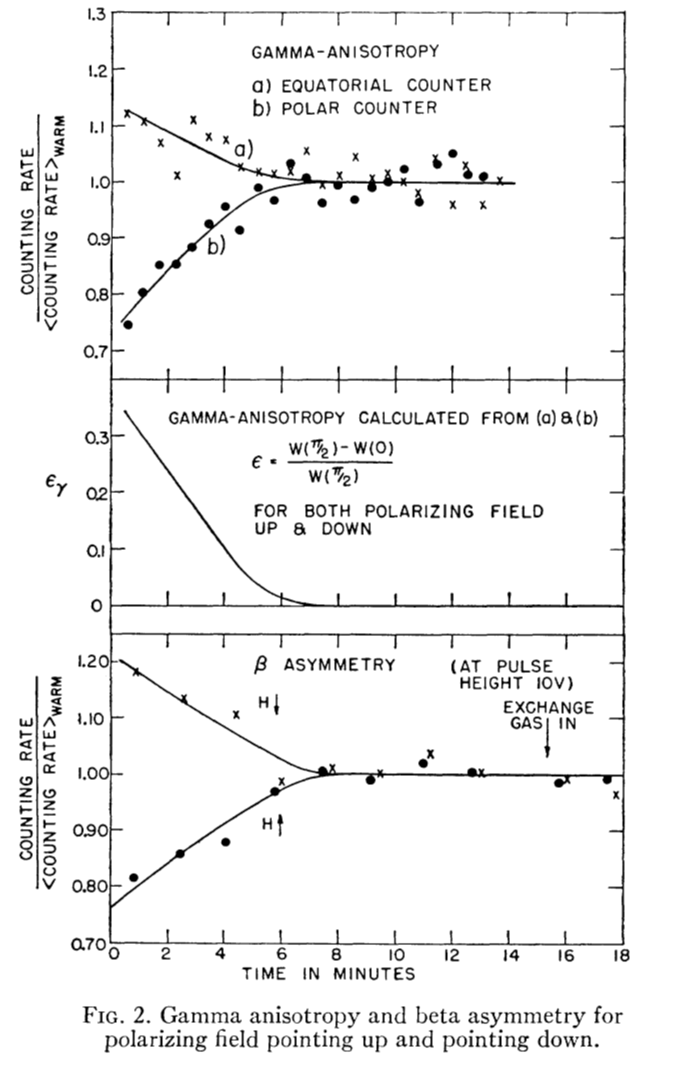
\includegraphics[width=10cm]{wu_expt.png}
  \caption{$\gamma$異方性と$\beta$非対称性の測定結果.どの図も$\ce{^60 Co}$のスピン偏光がなくなった時点を基準にとっている.}
  \label{fig:wu_expt}
\end{figure}

実験の結果,まず$\gamma$異方性は実験開始から約6分までの間観測された(図\ref{fig:wu_expt}上段,中段).
つまり,この時間内では核スピンは偏光していたことになる.
そして,$\beta$非対称性もこの時間内に観測され,カウント率は磁場が下向きのときは多く,磁場が上向きのときは多かった(図\ref{fig:wu_expt}下段).
この結果は($\gamma$異方性よりも)大きく非対称であり,電子は$\gamma$線すなわち核スピンと異なる方向に多く放出されることを意味している.
これが,弱い相互作用でパリティ対称性が破れていることの証明になった.

\begin{thebibliography}{99}
  \bibitem{wu_expt} Wu, C. S., Ambler E., Hayward R. W., Hoppes D. D., \& Hudson R. P., Experimental Test of Parity Conservation in Beta Decay, \textit{Physical Review}, 105(4): 1413-1415, 1957.
  \bibitem{wiki} Wu experiment - Wikipedia \\
  \url{https://en.wikipedia.org/wiki/Wu_experiment}
\end{thebibliography}